%\documentclass{report}\begin{document}
\chapter{Origin of the Cube}

\myTop{In this chapter we will describe the history behind \erno{} and how he got the idea for the \rubik{} in order to get a better understanding of the \rubik{}. Furthermore we will look at the development and the problematics describing the patenting and legal issues regarding the cube. We will look at the patent to get a better understanding of the cubes made at that time. The purpose of this chapter is to give the reader a basic understanding of the \rubik{}.}
\section{Ern\"{o} Rubik}
\erno{} is the inventor behind the world famous \rubik{}. He was born in Budapest, Hungary in 1944, his father was a flight engineer and his mother was a poet. He graduated from the Technical University in Budapest as an architectural engineer. After his graduation he stayed at the university to teach interior design.

In \myDate{}{1}{1975} Rubik applied for a patent for his invention in Hungary that was originally made to help his students. Two years later in 1977 he got the patent on the \mcube{}. This \mcube{} was actually the same cube as todays \rubik{}, he just named it differently. His \mcube{} should not be confused with the \mcube{} described in section \ref{sub:mcube}.
% Der er et spring fra Magic Cube til Rubiks Cube, som ikke beskrives

In the 1980's he became a professor and started the Rubik Studio, which employs a dozen people to design furniture and toys. 
Since the studios opening Rubik has produced several other toys, including Rubik's Snake. Most recently  the studio began developing computer games. 
He also became the president of the Hungarian Engineering Academy in 1990.The same year he created the International Rubik Foundation to support especially talented young engineers and industrial designers.

\begin{figure}
	\centering
		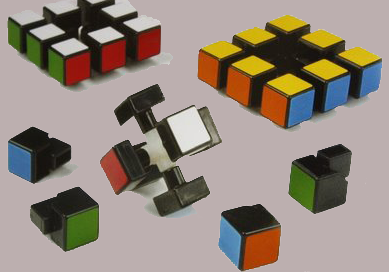
\includegraphics[scale=0.6]{input/pics/rubiks-cube.png}
	\caption{\myCaption{Figure of Rubik's Cube.}}
	\label{fig:rubiks-cube}
\end{figure}
 
\section{Rubik's Cube -- Magic Cube}

%In the 70s \erno{} was teaching Interior Design at Academy of Applied Arts and Crafts and he was trying to find a tool to help his students to understand three dimensional objects. As result he made the \mcube{} in 1974 and obtained a Hungarian patent HU170062. 
% Det ovenover er allerede beskrevet i forrige section

In the 1970's when \erno{} were teaching at the university he wanted to create a tool that would help his students to better understand tree-dimensional design. He wanted a design with blocks that could be moved individually, but also able to move several blocks at a time. Initially he attempted to do this with a cube held together by rubber bands. This failed. He then concluded after looking at a  Magic Puzzle (see chapter \ref{chap:recreationalMathematics}).
 that the pieces must hold each other in place. There by he created what was then called the \mcube{}. 

%Rubik described that some of the most important features behind the cube were that the parts of the cube stay together, which many other puzzles do not. He also pointed out that you can move several pieces at once. Also that it is three dimensional. 

In the end of 1970's a Hungarian Businessman showed the Magic Cube at the Nuremberg toy fair and made it popular in Europe. The company Ideal Toy bought exclusive rights for the Magic Cube, but changed the name of the cube to \rubik{} within a year in order to get trademark protection.

At that time there were also two others applying for patent for products similar to the \rubik{}.  One of them was an American man named Doctor Larry D. Nichols, and his cube was a 2x2x2 cube which was held together with magnets. See \ref{sec:nichols} .The other one who applied for patent was a Japanese man named Terutoshi Ishige. He applied for patent a year after Rubik. Terutoshi Ishige's cube was almost identically to the \rubik{}.

Ideal Toy Company were bought by CBS Toy Company in 1982 and the trademark surpassed with it, but they sold the rights to Rubik's Cube to Seven Towns which is a Toy Company in Great Britain, and they are still producing The Rubik's Cube today.

\section{The Nichols Cube Puzzle}
\label{sec:nichols}
Dr. Larry D. Nichols studied chemistry at DePauw University in Greencastle, Indiana, before moving to Massachusetts to attend Harvard Graduate School. 
He is a lifelong puzzle enthusiast and inventor who  began developing a twist cube puzzle with six colored faces in 1957. It was made of eight smaller cubes assembled to a 2x2x2 cube. The eight cubes were held together by magnets.

\begin{figure}[htb]
	\centering
		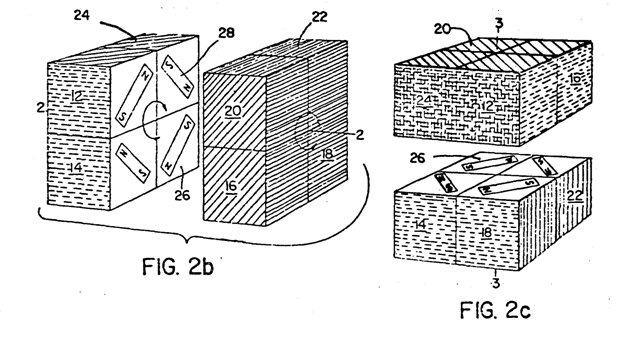
\includegraphics[scale=0.6]{input/pics/Nicholspatent2.png}
	\caption{\myCaption{Figure of Nichols Patent.}}
	\label{fig:Nicholspatent2}
\end{figure}

On \myDate{11}{4}{1972} he was granted U.S. Patent 3,655,201 on behalf of Moleculon Research Corp. U.S. Patent 3,655,201 covered Nichols Cube and the possibility for making larger versions later. This was two years before \erno{} took out the patent for his \rubik{} in Hungary. 

In 1982 Moleculon Research corp.  Sued Ideal Toy Company that had the U.S. Patent 4,378,116 for \rubik{} because they believed that Ideal Toy Company violated their patent, but the U.S. District Court ruled in Ideal Toy Company's favor. In 1986 the Court of Appeals ruled that the Pocket \rubik{} 2x2x2 was guilty of infringement but not the 3x3x3 \rubik{}. 

\chapter{The Upper and Lower Bounds}
\myTop{In this chapter we will describe the progress of the upper and lower bound of the \rubik{}.}

The lower bound is the number of twists required to solve the \rubik{} in the position which requires the most twists to solve.
The upper bound is the lowest number of twists proven to solve a \rubik{} in any position.
The different bounds through the history can be seen on figure \ref{fig:upperLowerBound}
%Both bounds can be seen on figure \ref{fig:upperLowerBound}.
As the figure shows, the upper bound closes in on the lower bound and at some point the two bounds will merge to one at some point.
%As the figure shows, the upper bound closes in on the lower bound.
%The graph show that the two lines will converge at some point.

\begin{comment}
A major breakthrough was when Thistlethwaite's algorithm was proven to be able to solve an arbitrary \rubik{} in 52 twists or less \cite{jaapthistle}.
Since then a lot of progress has been made in the field.
This section describes this progression.
\end{comment}

\begin{figure}[ht]
	\centering
		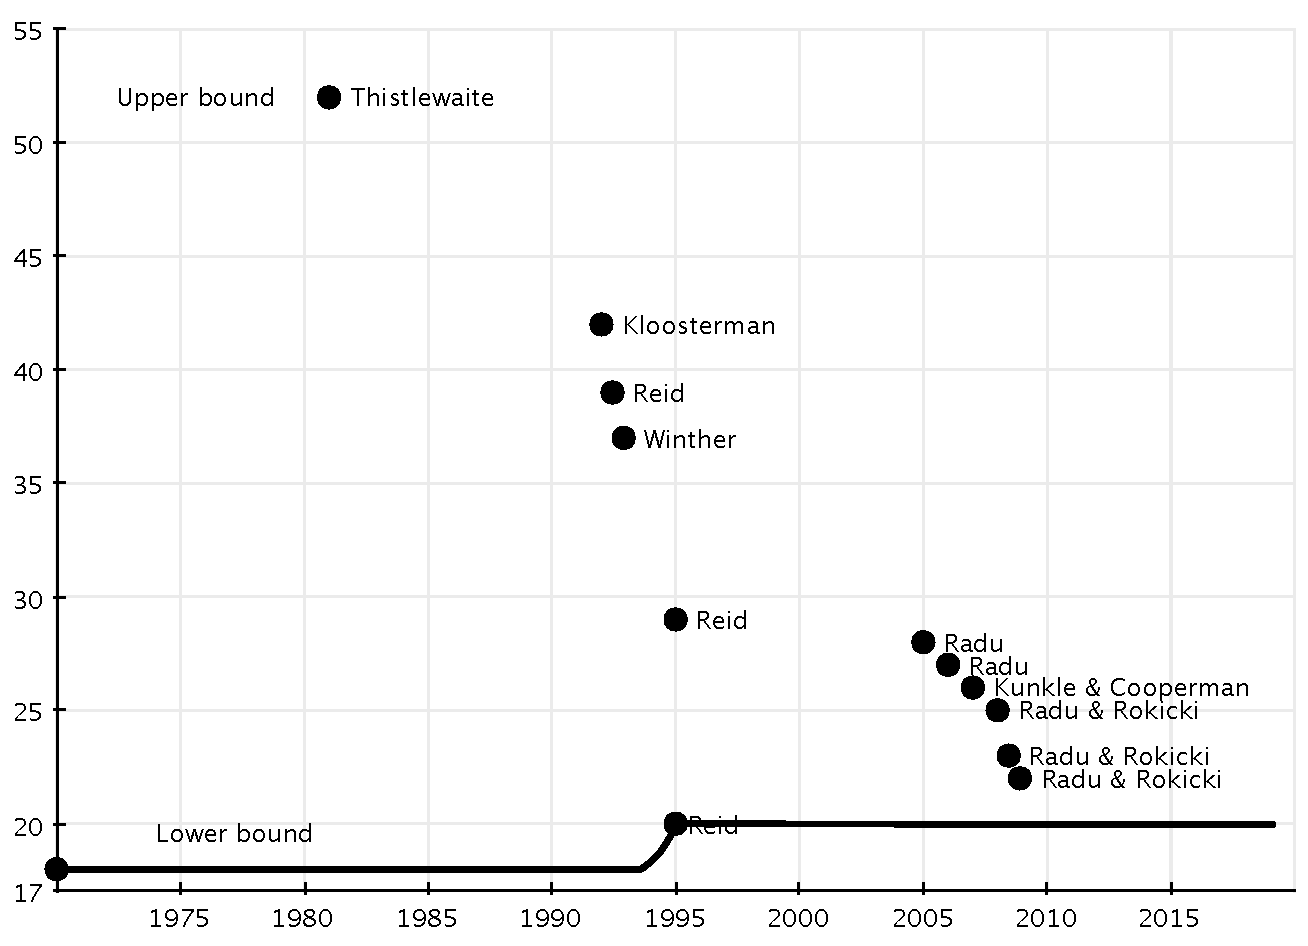
\includegraphics[scale = 0.7]{input/pics/bounds2.pdf}
	\caption{\myCaption{The current upper and lower bound. The x-axis depicts time and y-axis moves.}}
	\label{fig:upperLowerBound}
\end{figure}

\section{The Current and Previous Upper Bounds}
The progression of finding and proving the current and previous upper bounds have been a slow process.
%This is a slow moving field, but some events have occurred in the field the last couple of years.%% DAN DAN DAN DAN giv kilder pl0x
The reason why it is a slow process to prove the upper bound, is that there is a vast amount of different positions a \rubik{} can be in. Even with todays computer power there is simply to much data to process. This have inspired a small group of people to dedicate a lot of time to create and improve algorithms to solve arbitrary \rubik{}s.
%the effect that a small group of people dedicate a lot of time to create and improve algorithms to solve arbitrary \rubik{}s. 

\begin{comment}

The set solver created by Thomas Rockicki, which was described in the previous section will now be further described.

%The result

The set solver has a special way of testing the \rubik{}s. It does not solve them to the unit position $e$, instead it finds a move sequence for a subgroup of the \rubik{} this way it can solve approximately 19.5 billion cubes at a time and not just one. The reason for this is that if you relabel an arbitrary cube, that given cube can be unlabeled to approximately 19.5 billion different cube positions. Recall that there are approximately 19.5 billion positions in the set \m{H} and all these positions are equal to $e$ when relabeled. The same logic applies to any other given position.
\end{comment}

Proofs of the upper bound has been published several times, and it has been lowered each time.
The first to find \textit{God's algorithm} was Thistlethwaite. Thistlethwaite's algorithm was proven to be able to solve an arbitrary \rubik{} in 52 twists or less \cite{jaapthistle}.
\emph{SOMETHING ABOUT HIS ALGORITHM!!!}

This upper bound existed in over 10 years and the next upper bound was found in 1992 by Hans Kloosterman, which reduced the upper bound to 42 moves %\cite{rokickipdf}. 
He modified Thistlethwaite's algorithm and founds some shortcuts to reduce the moves by replacing the \m{G3} subgroup with a different subgroup and removed a move between stage 3 and 4.

In May 1992, Michael Reid reduced the upper bound to 39 moves by using a three phase algorithm and a thorough analysis of the groups.

One day after Michael Reid, Dik Winter reduced the upper bound to 37 moves

\begin{comment}
The progression greatly accelerated when that set solver proved the first upper bound of 25 moves. This was done on home computers from October 2007 to March 2008. They only needed to solve 6000 sets, but after this they got contacted by John Welborn from Sony Pictures Imageworks and he offered a lot of idle computers from a computer farm to help on the project. 
\end{comment}
After this the process of lowering the bound sped up, not long after they proved the upper bound of 24 and 23. As the upper bound is lowered they need to solve more and more sets to ensure that it is the upper bound, and they needed to test almost 27000 and 180000 sets for 24 and 23. 


The current upper bound is on 22 moves and was proved in 2009 \cite{rokicki09}. To prove this they needed to compute 1,265,326 different sets. At the moment they have not proven that the upper bound can be 21, but the computer farm is currently working on it, and they expect that it is possible to lower the upper bound to 20. This means that any arbitrary \rubik{} could be solved in just 20 moves.

\subsection{The Lower Bound}
As mentioned previously in this chapter the lower bound is the number of twists required to solve the \rubik{} in the position which requires the most twists to solve. 
For now it is proven that the superflip position(see figure \ref{fig:superflip}), is the position which requires the most twists to be solved \cite{speedsolving.wiki}.
The shortest path from the superflip to the solved position is 20 twists \cite{rokicki09}.
This has been proven by trying every possible solutions with 19 twists or less. 
There has not been found a position that requires more than 20 twists, which makes the lower bound 20 twists.

\begin{figure}[ht]
	\centering
		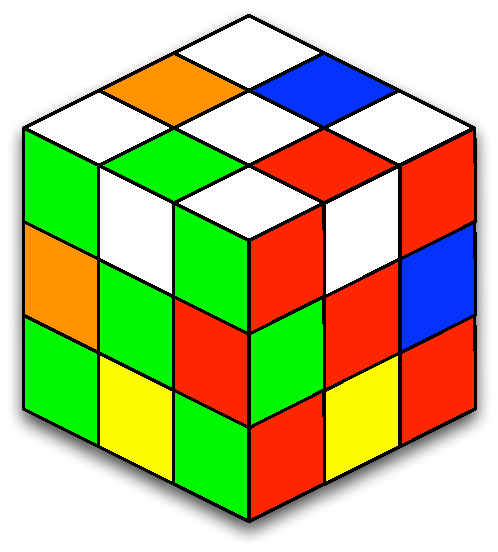
\includegraphics[scale = 0.7]{input/pics/superflip.pdf}
	\caption{\myCaption{The superflip: every edge is flipped. The optimal solution to this position is 20 twists.}}
	\label{fig:superflip}
\end{figure}





\myTail{noget andet}

\myTail{In this chapter it has been described how \erno{} got the idea for the cube. We also stated that \erno{} was not the only one at that time, that came with the invention of cubes. \erno{}'s cube was special since the blocks hold each other together, which is different from the one Doctor Larry D. Nichols applied patent for which is hold together with magnets. 
}
%\end{document}